% §5 The Bravyi–Kitaev Encoding and Fenwick Trees
%
% Explains how BK actually works, the Fenwick tree, and why
% it is NOT a generic tree-to-index-set instance.

The Bravyi--Kitaev (BK) encoding~\cite{bravyi2002, seeley2012}
achieves $O(\log_2 n)$ Pauli weight by using a tree-structured storage
scheme for partial parities.  Understanding how BK is constructed is
essential to understanding the star-tree theorem's implications.

\subsection{The Fenwick tree}
\label{sec:fenwick-tree}

The BK encoding is built on the Fenwick tree (also called a binary
indexed tree)~\cite{fenwick1994}, a data structure originally designed
for efficient prefix-sum computation.

\begin{definition}[Fenwick tree]
\label{def:fenwick-tree}
For $n$ nodes indexed $\{0, \ldots, n{-}1\}$, the \emph{Fenwick tree}
is the rooted tree where the parent of node~$j$ (for $j > 0$) is
$j + \mathrm{lsb}(j)$, where $\mathrm{lsb}(j)$ is the least
significant bit of~$j$ (i.e., $j \mathbin{\&} (-j)$).    The root is the
node with the largest index that is a power of~2 (or $n$ rounded up).
\end{definition}

For $n = 8$, the Fenwick tree is:
\begin{center}
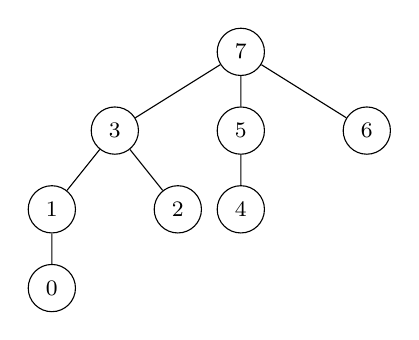
\begin{tikzpicture}[
  level distance=10mm, sibling distance=16mm,
  every node/.style={circle,draw,minimum size=6mm,inner sep=0pt,
    font=\footnotesize}
]
\node {7}
  child { node {3}
    child { node {1}
      child { node {0} }
    }
    child { node {2} }
  }
  child { node {5}
    child { node {4} }
  }
  child { node {6} };
\end{tikzpicture}
\end{center}

The tree has depth $O(\log_2 n)$, and each node stores the partial
parity of a specific range of mode occupations determined by the
binary structure of its index.

\subsection{BK index sets via bit manipulation}
\label{sec:bk-bit-formulas}

The BK encoding derives its index sets using bit-manipulation
formulas specific to the Fenwick tree's structure:

\begin{align}
  U(j) &= \{j + \mathrm{lsb}(j),\; j + \mathrm{lsb}(j) +
    \mathrm{lsb}(j + \mathrm{lsb}(j)),\; \ldots\},
    \label{eq:bk-update} \\
  P(j) &= \{j - 1,\; j - 1 - \mathrm{lsb}(j-1),\; \ldots\},
    \label{eq:bk-parity} \\
  \mathrm{Occ}(j) &= \{j,\; j - \mathrm{lsb}(j),\;
    j - \mathrm{lsb}(j) - \mathrm{lsb}(j - \mathrm{lsb}(j)),\;
    \ldots\}.
    \label{eq:bk-occ}
\end{align}

These formulas produce $O(\log_2 n)$-sized sets, yielding the
logarithmic Pauli weight that makes BK attractive.

\subsection{Construction F: Fenwick-specific, not generic}
\label{sec:construction-f}

A crucial observation for the star-tree theorem:
the BK index sets~\eqref{eq:bk-update}--\eqref{eq:bk-occ} are
\emph{not} the same as applying the generic tree-derived
formulas~\eqref{eq:tree-derived-sets} to a Fenwick-shaped tree.

\begin{keyinsight}
The Bravyi--Kitaev encoding uses hand-derived bit-manipulation
formulas (which we call \emph{Construction~F}) that exploit the
unique algebraic structure of the Fenwick tree.  These formulas
produce a valid encoding, but they are algebraically distinct from
the generic \emph{tree-to-index-set} derivation
(Construction~A, \cref{sec:tree-derived}) applied to the same tree
shape.
\end{keyinsight}

To see the distinction concretely, consider applying
Construction~A's generic formula~\eqref{eq:tree-derived-sets} to
the Fenwick tree on $n = 8$.  The generic formula reads off
ancestors, children, and descendants from the tree structure.  The
resulting index sets differ from the BK bit-manipulation formulas,
and --- as we prove in \cref{sec:star-tree} --- the generic sets
\emph{violate the CAR} because the Fenwick tree has depth~$> 1$.

The SRL paper~\cite{seeley2012} presents both JW/Parity and BK as
instances of its index-set framework.  This is technically correct:
BK \emph{can be expressed} as an index-set scheme (one can always
write down the three sets).  But the framework elides a key
distinction: for JW and Parity, the sets are mechanically derivable
from a star tree, while for BK, they are obtained via a separate,
Fenwick-specific computation.

\subsection{BK in practice}

Despite this conceptual distinction, BK remains highly useful:
\begin{itemize}
  \item Pauli weight $O(\log_2 n)$, a major improvement over JW.
  \item Straightforward implementation via bit-manipulation.
  \item Widely supported in quantum chemistry software
    (OpenFermion~\cite{mcclean2020}, Qiskit~\cite{qiskit2023},
    PennyLane~\cite{bergholm2022}).
\end{itemize}

The star-tree theorem does not invalidate BK --- it clarifies which
construction \emph{produces} BK.  BK is valid because Construction~F
is valid, not because it is a generic tree-to-index-set instance.
